% Created 2017-04-16 Sun 20:39
% Intended LaTeX compiler: pdflatex
\documentclass[a4paper,11pt]{article}
\usepackage[utf8]{inputenc}
\usepackage[T1]{fontenc}
\usepackage{graphicx}
\usepackage{grffile}
\usepackage{longtable}
\usepackage{wrapfig}
\usepackage{rotating}
\usepackage[normalem]{ulem}
\usepackage{amsmath}
\usepackage{textcomp}
\usepackage{amssymb}
\usepackage{capt-of}
\usepackage{hyperref}
\usepackage[margin=1in]{geometry}
\usepackage{setspace}
\onehalfspacing
\usepackage{parskip}
\usepackage{mathtools}
\usepackage{hyperref}
\hypersetup{colorlinks,citecolor=black,filecolor=black,linkcolor=black,urlcolor=black}
\usepackage{graphicx}
\usepackage{tabularx}
\usepackage{color}
\usepackage[font={footnotesize}]{caption}
\newtheorem{mydef}{Definition}
\newtheorem{mythm}{Theorem}
\newcommand{\dx}{\mathrm{d}}
\newcommand{\var}{\mathrm{Var}}
\newcommand{\cov}{\mathrm{Cov}}
\newcommand{\corr}{\mathrm{Corr}}
\newcommand{\pr}{\mathrm{Pr}}
\newcommand{\rarrowd}[1]{\xrightarrow{\text{ \textit #1 }}}
\DeclareMathOperator*{\plim}{plim}
\newcommand{\plimn}{\plim_{n \rightarrow \infty}}
\setcounter{secnumdepth}{2}
\author{Zheng Tian}
\date{}
\title{Lecture 1. Review on Linear Time Series Models}
\hypersetup{
 pdfauthor={Zheng Tian},
 pdftitle={Lecture 1. Review on Linear Time Series Models},
 pdfkeywords={},
 pdfsubject={},
 pdfcreator={Emacs 25.1.1 (Org mode 9.0.3)}, 
 pdflang={English}}
\begin{document}

\maketitle
\setcounter{tocdepth}{2}
\tableofcontents



\section{Introduction}
\label{sec:org2bbc387}

This lecture reviews what we have learned about the linear time series
models, namely, AR, MA, and ARMA models. These models are the
foundation of what we are going to learn in the following lectures. The
review is far from comprehensive but gives you a big picture regarding
these models and links them with what to be learned next.


\section{Financial Time Series Data}
\label{sec:org511a9a9}

This course mainly concerns time-series data of the returns to
financial assets. Let \(P_t\) be the price of an financial asset at time
\(t\). Then, what we are mostly interested is the following

\[ r_t = ln(P_t) - ln(P_{t-1}) \]

\(\{r_t\}\) is the series of asset returns for \(t = 1, \ldots, T\).


\section{Weak Stationarity}
\label{sec:org7fd5e26}

The foundation of time series analysis is the concept of stationarity. Mostly, we
focus on \textbf{weak stationarity}.

A series \(\{r_t\}\) is weakly stationary if
\begin{enumerate}
\item \(E(r_t) = \mu < \infty\) where \(\mu\) is a constant
\item \(\cov(r_t, r_{t-\ell}) = \gamma_{\ell} < \infty\), which only depends on \(\ell\).
\end{enumerate}

It follows that \(\var(r_t) = \gamma_0 < \infty\), which is also a
constant.


\section{The ACF and the Ljung-Box Test}
\label{sec:org9d00fa4}

We can use \textbf{the autocorrelation function (ACF)} to characterize the
influence of the past value of the series \(r_{t-i}\) for \(i = 1,
\ldots, T\) on the current value \(r_t\).

\begin{itemize}
\item The \textbf{lag-\(\ell\) ACF} of the series \(\{r_t\}\) is
\[ \rho_{\ell} = \frac{\cov(r_t, r_{t-\ell})}{\sqrt{\var(r_t)\var(r_{t-\ell})}} = \frac{\gamma_{\ell}}{\gamma_0} \]

\item The \textbf{sample lag-\(\ell\) ACF} is computed as
\[ \hat{\rho}_{\ell} = \frac{\sum_{t=\ell+1}^T (r_t -
  \bar{r})(r_{t-\ell} - \bar{r})}{\sum_{t=1}^T (r_t - \bar{r})^2},\; 0
  \leq \ell < T-1 \]

Note that when defining ACF, we implicitly assume \(r_t\) is weakly
stationary.

\item When \{\(r_t\)\} is weakly stationary, say an ARMA proess, then we know
the asymptotic distribution is 
\[ \hat{\rho}_{\ell} \sim N \left(0, \frac{1}{T}(1+2\sum_{i=1}^q
  \hat{\rho}_i^2) \right) \text{ for } \ell > q \]

\item The \textbf{Ljung-Box test} is commonly used to test the existence of
autocorrelation in \(\{r_t\}\).

The null hypothesis is
\[ H_0: \rho_1 = \cdots = \rho_m = 0,\; H_1: \rho_i \neq 0 \text{
  for some } i \in \{1, \ldots, m\} \]

The test statistic is
\[ Q(m) = T(T+2)\sum_{\ell=1}^m \frac{\hat{\rho}^2_{\ell}}{T-\ell}
  \sim \chi^2(m) \]
When \(Q(m) > \chi^2_{\alpha}\), where \(\chi^2_{\alpha}\) is the
critical value at the significance level of \(\alpha\) of a
chi-squared distribution with \(m\) degree of freedom.

We often use correlogram to display the ACF of a series. Figure
\ref{fig:orge098069} shows the ACF of the monthly return of IBM
stock. 
\begin{itemize}
\item The sample ACFs are all within their two standard error
limits, indicating that they are not significantly different from
zero at the 5\% level.
\item For the simple returns, the Ljung–Box statistics give \(Q(5) =
    3.37\) and \(Q(10) = 13.99\), which correspond to p values of 0.64
and 0.17, based on the chi-squared distributions with 5 and 10
degrees of freedom.
\item For the log returns, we have \(Q(5) = 3.52\) and \(Q(10) = 13.39\)
with p values 0.62 and 0.20, respectively.
\end{itemize}
The joint tests confirm that monthly IBM stock returns have no
significant serial correlations.

\begin{figure}[htbp]
\centering
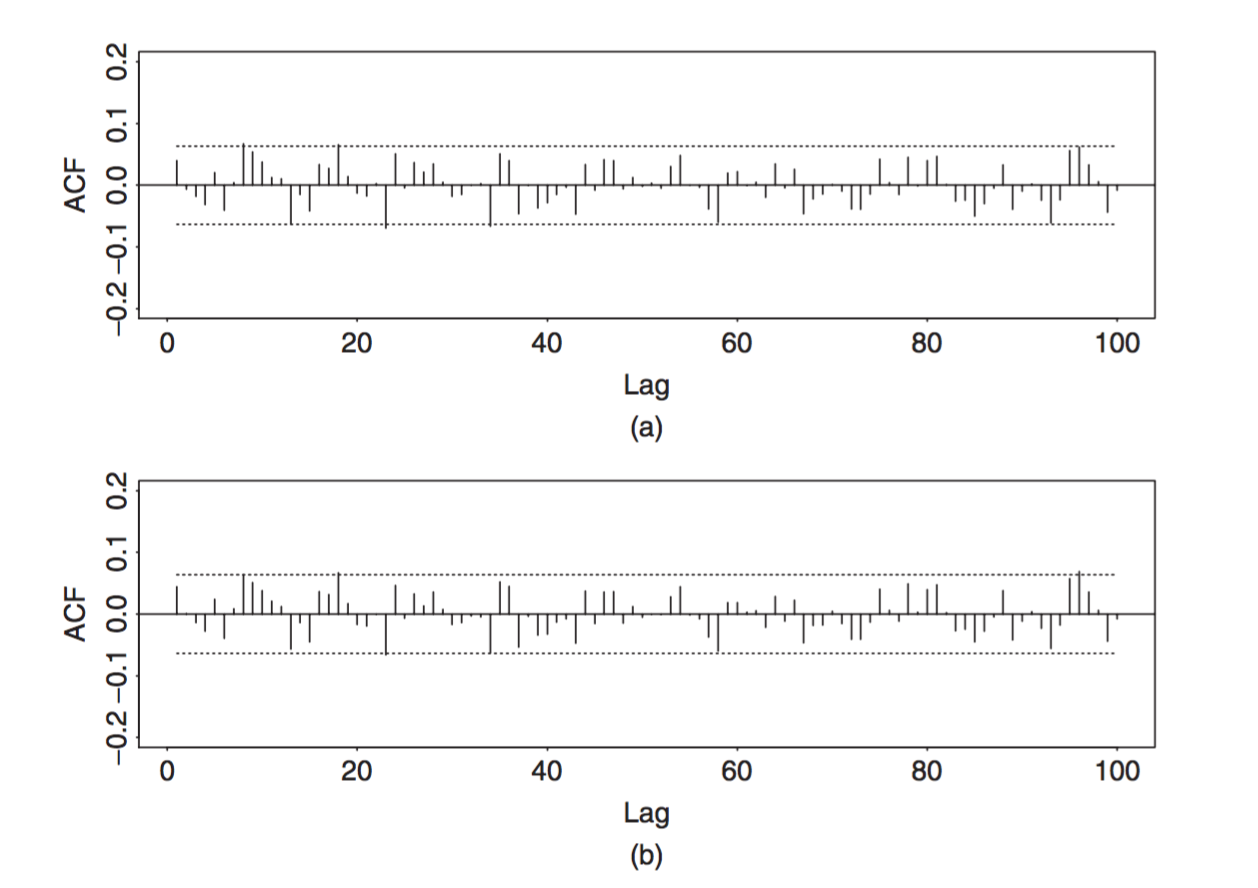
\includegraphics[width=0.8\textwidth]{img/ibm_return.png}
\caption{\label{fig:orge098069}
Sample autocorrelation functions of monthly (a) simple returns and (b) log returns of IBM stock from January 1926 to December 2008. In each plot, two horizontal dashed lines denote two standard error limits of sample ACF}
\end{figure}
\end{itemize}


\section{The Linear Time Series Models}
\label{sec:org2bdb131}

\subsection{The ARMA Model}
\label{sec:org2df0fcf}

Autoregressive moving-average models \(\mathrm{ARMA}(p, q)\)
encompass autoregressive models \(\mathrm{AR}(p)\) and
moving-average models \(\mathrm{MA}(q)\).

A general \(\mathrm{ARMA}(p, q)\) model is in the form of
\begin{equation}
\label{eq:armapq}
r_t = \phi_0 + \sum_{i=1}^p \phi_i r_{t-i} + a_t - \sum_{i=1}^q \theta_i a_{t-i}
\end{equation}
where \(\{a_t\}\) is a white noise series, i.e., \(a_t \sim
\mathrm{i.i.d.}(0, \sigma^2_a)\).

From the general \(\mathrm{ARMA}(p, q)\) model, we know that \(\mathrm{AR}(p)\) models are
simply \(\mathrm{ARMA}(p, 0)\) and \(\mathrm{MA}(q)\) models are \(\mathrm{ARMA}(0, q)\) for \(p, q >
0\).

What we are interested in these models can be summarized by the
following items:
\begin{itemize}
\item The stationarity condition
\item The statistical properties
\begin{itemize}
\item The (un)conditional mean, \(E(r_t)\)
\item The (un)conditional variance, \(\var(r_t)\).
\item The ACF, \(\rho_{\ell}\) for \(\ell > 0\).
\end{itemize}
\item Estimation and model checking
\item Forecasting
\end{itemize}


\subsection{The Stationarity Condition}
\label{sec:org66c3c13}

\begin{itemize}
\item The \textbf{characteristic equation} of all \(\mathrm{ARMA}(p, q)\) models
comes from the homogeneous part of Equation \eqref{eq:armapq}, that
is, 
\[ r_t - \phi_1 r_{t-1} - \cdots - \phi_p r_{t-p} = 0  \]

Therefore, the characteristic equation is
\begin{equation}
\label{eq-chareq}
\alpha^p - \phi_1 \alpha^{p-1} - \cdots - \phi_p = 0
\end{equation}
The solutions to this equation are the \textbf{characteristic roots}.

\item The weak stationarity requires that \textbf{the characteristic roots be less
than one in modulus} (i.e., they are within a unit circle).
\begin{itemize}
\item If the root is a real number, \(\alpha\), then weak stationarity
requires \(|\alpha| < 1\).
\item If the root is a complex number, \(\alpha = a + bi\) where \(i =
    \sqrt{-1}\), then weak stationarity requires \(r = \sqrt{a^2 + b^2} < 1\).
\end{itemize}

\item \(\mathrm{AR}(p)\) and \(\mathrm{ARMA}(p,q)\) share the same
characteristic equation as Equation \eqref{eq-chareq} so that their
stationarity conditions are also the same.

\item \(\mathrm{MA}(q)\) models are always weakly stationary as long as the
\(\{a_t\}\) series is white noise.
\end{itemize}


\subsection{The AR Model}
\label{sec:orgc235294}

\subsubsection*{The simple \(\mathrm{AR}(1)\) model}
\label{sec:org3437d03}

We review the properties of \(\mathrm{AR}(p)\) model using the simple
\(\mathrm{AR}(1)\) process,
\begin{equation}
\label{eq-ar1}
r_t = \phi_0 + \phi_1 r_{t-1} + a_t,\; a_t \sim i.i.d.(0, \sigma^2_a)
\end{equation}

\subsubsection*{The stationarity condition}
\label{sec:org5fcd408}

The characteristic equation of Equation \eqref{eq-ar1} is
\[ \alpha - \phi_1 = 0 \]
The characteristic root is simply \(\alpha = \phi_1\). Thus, the
stationarity condition of an \(\mathrm{AR}(1)\) process is
\(|\phi_1|<1\).

Remember that when we derive the unconditional mean, variance and ACF
of \(r_t\), we always assume that \(\{r_t\}\) is weakly stationary that is
\(|\phi_1| < 1\).

\subsubsection*{The expectations}
\label{sec:org6de6ab9}

\begin{itemize}
\item The unconditional mean of \(r_t\) is
\[ E(r_t) = \mu = \frac{\phi_0}{1 - \phi_1} \]
Because \(\{r_t\}\) is weakly stationary, its mean is constant over
time.

\item The conditional mean of \(r_t\) given the information at \(t-1\) is
\[ E(r_t \mid r_{t-1}) = \phi_0 + \phi_1 r_{t-1} \]
\end{itemize}

\subsubsection*{The variance}
\label{sec:org89f00a8}

\begin{itemize}
\item The unconditional variance of \(r_t\) is
\[ \var(r_t) = \frac{\sigma^2_a}{1 - \phi_1^2} \]
The unconditional variance is also a constant because of weak
stationarity. The existence of the unconditional mean and variance
of \(r_t\) requires \(|\phi_1| < 1\), which is also the sufficient
condition for weak stationarity.

\item The conditional variance of \(r_t\) given \(r_{t-1}\) is
\[ \var(r_t \mid r_{t-1}) = \var(a_t) = \sigma^2_a \]
\end{itemize}

\subsubsection*{The ACF}
\label{sec:org8776cc1}

The ACF of \(\mathrm{AR}(1)\) is
\[\rho_0 = 1,\; \rho_{\ell} = \phi_1 \rho_{\ell-1}, \text{ for }
\ell>0 \]
It says that the ACF of a weakly stationary AR(1) series decays
exponentially with rate \(\phi_1\) and starting value \(\rho_0=1\).

\begin{figure}[htbp]
\centering
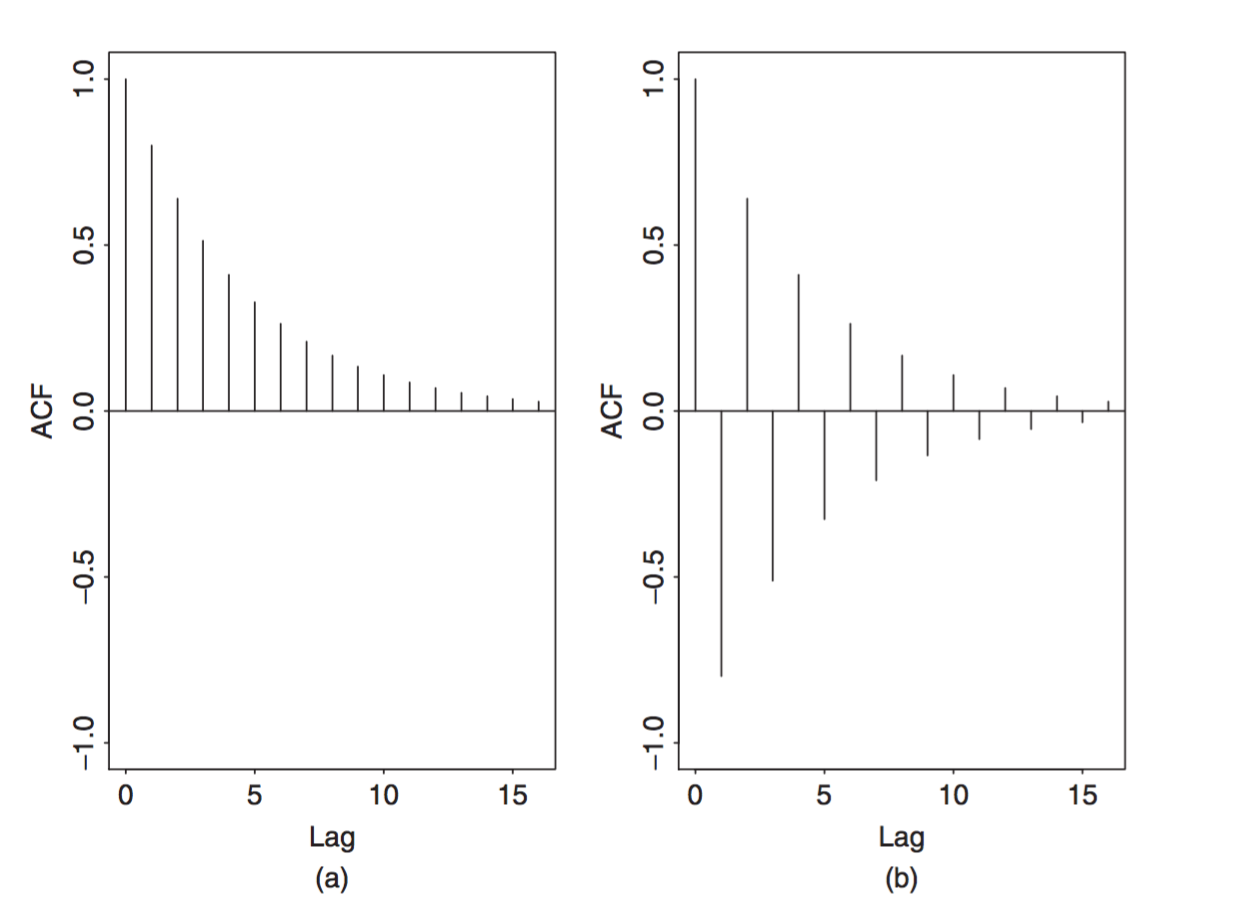
\includegraphics[width=0.8\textwidth,height=0.3\textheight]{img/acf_ar1.png}
\caption{\label{fig:org826f11a}
Autocorrelation function of an AR(1) model: (a) for \(\phi_1 = 0.8\) and (b) for \(\phi_1 = −0.8\)}
\end{figure}

\subsubsection*{The ACF for the general AR(p) model}
\label{sec:org98d7710}

For a general \(AR(p)\) model,
\begin{equation}
\label{eq-arp}
r_t = \phi_0 + \sum_{i=1}^p \phi_i r_{t-i} + a_t,\; a_t \sim i.i.d.(0, \sigma^2_a)
\end{equation}

\begin{itemize}
\item The unconditional mean is
\[ E(r_t) = \frac{\phi_0}{1 - \sum_{i=1}^p \phi_i} \]

\item The ACF of \{\(r_t\)\} is governed by the following difference equation
\[ \rho_{\ell} = \phi_1 \rho_{\ell-1} + \phi_2 \rho_{\ell-2} +
  \cdots + \phi_p \rho_{\ell-p} \]
Rewritten with the lag operator \(L\), we have
\[ (1 - \phi_1 L - \cdots - \phi_p L^p) \rho_{\ell} = 0 \]
where \(1 - \phi_1 L - \cdots - \phi_p L^p=0\) is the inverse
characteristic equation.

\item An \(\mathrm{AR}(p)\) series is weakly stationary when all the roots
of the inverse characteristic equation are greater than one in
modulus.
\end{itemize}

\subsubsection*{Estimation and model checking of \(\mathrm{AR}(p)\) models}
\label{sec:org3a68f9e}

\begin{itemize}
\item We can use the sample ACF, the sample PACF (partial ACF), AIC, and BIC to determine the order of the
AR process. Especially, the PACF of an \(\mathrm{AR}(p)\) series exhibits a
noticeable cut-off towards zero at the lag \(\ell\) for \(\ell > p\).

\item We use the ordinary least squares (OLS) method to estimate an
\(\mathrm{AR}(p)\) model with the appropriate order \(p\).

\item We use the Ljung-Box test to check whether the residual series
\{\(\hat{a}_t\)\} is a white noise series.
\end{itemize}

\subsubsection*{Forecasting}
\label{sec:org5358beb}

The \(\ell\)-step-ahead forecast at time \(h\) is
\[ \hat{r}_h(\ell) = \phi_0 + \sum_{i=1}^p \phi_i \hat{r}_h(\ell-i) \]

The stationary \(\mathrm{AR}(p)\) model is said to be \textbf{mean reversion}
because as \(\ell \rightarrow \infty\), \(\hat{r}_h(\ell) \rightarrow
E(r_t)\).


\subsection{The MA Model}
\label{sec:orgc03f1be}

\subsubsection*{The simple \(\mathrm{MA}(1)\) model}
\label{sec:org9477336}

The simple \(\mathrm{MA}(1)\) model takes the form as
\begin{equation}
\label{eq-ma1}
r_t = c_0 + a_t - \theta_1 a_{t-1},\; a_t \sim i.i.d.(0, \sigma^2_a)
\end{equation}

\subsubsection*{The stationarity condition}
\label{sec:org4259738}

An \(\mathrm{MA}(1)\) series is always weakly stationary. That is because
\begin{itemize}
\item \(E(r_t) = c_0\) is a constant;
\item \(\gamma_0 = \var(r_t) = (1 + \theta_1^2) \sigma^2_a\)
\item \(\gamma_1 = \cov(r_t, r_{t-1}) = -\theta_1 \sigma^2_a,\;
  \gamma_{\ell} = 0, \text{ for } \ell>0\).
\end{itemize}

\subsubsection*{The ACF}
\label{sec:orgb4b70e8}

The ACF of \(\mathrm{MA}(1)\) is
\[\rho_0 = 1,\; \rho_1 = -\frac{\theta_1}{1+\theta^2_1},\; \rho_{\ell}
= 0, \text{ for } \ell>1 \]

\subsubsection*{The general \(\mathrm{MA}(q)\) model}
\label{sec:orgaa8b20a}

The general \(\mathrm{MA}(q)\) model is
\begin{equation}
\label{eq-maq}
r_t = c_0 + a_t - \sum_{i=1}^q \theta_i a_{t-i},\; a_t \sim i.i.d.(0, \sigma^2_a)
\end{equation}

An \(\mathrm{MA}(q)\) model is always weakly stationary. The ACFs from
lag 1 to lag q are not zero, while \(\rho_{\ell} > 0\) when \(\ell > q\).

\subsubsection*{Estimation and model checking}
\label{sec:org8b76449}

\begin{itemize}
\item Use the sample ACF to determine the order of \(\mathrm{MA}(q)\).

\item \(\mathrm{MA}(q)\) models can be estimated using either the
conditional maximum likelihood method or the exact maximum
likelihood method.

\item Use the Ljung-Box test to check whether the residuals are white
noise.
\end{itemize}

\subsubsection*{Forecasting}
\label{sec:org9352721}

For an \(\mathrm{MA}(1)\) model, the \(\ell\)-step-ahead forecast is
\begin{align*}
\hat{r}_h(1) &= c_0 - \theta_1 a_{h-1} \\
\hat{r}_h(\ell) &= 0 \text{ for } \ell > 1
\end{align*}
That is, the forecasts go to the mean of \{\(r_t\)\} after 1 step.

For an \(\mathrm{MA}(q)\) model, the \(\ell\)-step-ahead forecasts go to
the mean after the first q steps.


\subsection{The ARMA Model}
\label{sec:org8cd90ac}

\subsubsection*{The simple \(\mathrm{ARMA}(1,1)\) model}
\label{sec:org25f564d}

A time series \{\(r_t\)\} follows an \(\mathrm{ARMA}(1,1)\) model if it
satisfies
\begin{equation}
\label{eq-arma11}
r_t = \phi_0 + \phi_1 r_{t-1} + a_t - \theta_1 a_{t-1}
\end{equation}
where \{\(a_t\)\} is a white noise series.

\subsubsection*{The expectation and variance of \(\mathrm{ARMA}(1,1)\)}
\label{sec:org6985de6}

\begin{itemize}
\item The unconditional expectation of an \(\mathrm{ARMA}(1, 1)\) series is
\[E(r_t) = \frac{\phi_0}{1 - \phi_1}\]

\item The unconditional variance is
\[ \gamma_0 = \var(r_t) = \frac{(1-2\phi_1 \theta_1 + \theta_1^2) \sigma^2_a}{1-\phi_1^2} \]
\end{itemize}

\subsubsection*{The ACF of \(\mathrm{ARMA}(1,1)\)}
\label{sec:org8e5480d}

The ACF of an \(\mathrm{ARMA}(1,1)\) series is governed by the following
difference equation
\[ \rho_0 = 1,\; \rho_1 = \phi_1 - \frac{\theta_1
\sigma^2_a}{\gamma_0},\; \rho_{\ell} = \phi_1 \rho_{\ell-1}, \text{
for } \ell>1 \]

The ACF exhibits a similar pattern to an \(\mathrm{AR}(1)\) model except
that the exponential decay starts with lag 2 instead of lag 1.

\subsubsection*{The estimation, model checking, and forecasting}
\label{sec:orgffd1bdb}

\begin{itemize}
\item The order of an \(\mathrm{ARMA}(p,q)\) model can be determined by EACF
(extended ACF), AIC, and BIC.
\item The estimation method is either the conditional likelihood method or
the exact likelihood method.
\item The Ljung-Box test is used to check whether the residual series is a
white noise series.
\item The \(\ell\)-step-ahead forecast is
\[ \hat{r}_h(\ell) = E(r_{h+\ell} \mid F_h) = \phi_0 + \sum_{i=1}^p
  \phi_i \hat{r}_h(\ell-i) - \sum_{i=1}^q \theta_i a_h(\ell-i) \]
\end{itemize}


\section{Random Walk and Unit-Root Nonstationarity}
\label{sec:orgc78cfd0}

The AR, MA, and ARMA models are all models for stationary time series,
whereas not all time series data are stationary. Next, we review the
models for unit-root nonstationary data, including random walk, random
walk with a drift, the trend-stationary model, and \(\mathrm{ARIMA}(p, d, q)\).

\subsection{Random Walk and Random Walk with a Drift}
\label{sec:org112b9bc}

Consider the following models
\begin{align}
p_t &= \phi_1 p_{t-1} + e_t  \label{eq:ar1a} \\
p_t &= \mu + \phi_1 p_{t-1} + e_t \label{eq:ar1b}
\end{align}
When \(|\phi_1| < 1\), we know that both Equations (\ref{eq:ar1a}) and
(\ref{eq:ar1b}) are stationary \(\mathrm{AR}(1)\) processes.

If \(\phi_1 = 1\), then Equation (\ref{eq:ar1a}) turns to a \textbf{random
walk} model, and Equation (\ref{eq:ar1b}) turns to a \textbf{random walk with
a drift} model. Since \(\phi_1\) is the root of the characteristic
equations for Equations (\ref{eq:ar1a}) and (\ref{eq:ar1b}), the random
walk and random walk with a drift models are all \textbf{unit-root}
nonstationary models.

\subsubsection*{Random walk}
\label{sec:orgc293fb2}

The log price of a stock usually follows a random walk process.
\begin{equation}
\label{eq:randwalk}
p_t = p_{t-1} + a_t,\; a_t \sim i.i.d.(0, \sigma^2_a)
\end{equation}

\begin{itemize}
\item The MA representation of Equation (\ref{eq:randwalk}) is
\[ p_t = p_0 + a_t + a_{t-1} + \cdots + a_1 \]
which implies that the past shocks have permanent non-diminishing
effects on the current price.

\item The \(\ell\)-step-ahead forecast is
\[ \hat{p}_h(\ell) = E(p_{h+\ell} \mid p_h, p_{h-1}, \ldots) = p_h,
  \text{ for } \ell > 0 \]
It says that for all forecast horizons, the point forecasts of a
random-walk model are simply the value of the series at the forecast
origin.

\item The forecast error is
\[ e_h(\ell) = a_{h+\ell} + \cdots + a_{h+1} \]
of which \(\var[e_h(\ell)] = \ell \sigma^2_a\). It implies that the
forecast errors will increase infinitely as \(\ell \rightarrow \infty\).
\end{itemize}

\subsubsection*{Random walk with a drift}
\label{sec:orgcd3bb14}

A random walk series with a drift takes the following form
\begin{equation}
\label{eq:randwalkdr}
p_t = \mu + p_{t-1} + a_t,\; a_t \sim i.i.d.(0, \sigma^2_a)
\end{equation}

\begin{itemize}
\item The existence of \(\mu\) add a time trend to \{\(p_t\)\}. That is, we can
rewrite Equation (\ref{eq:randwalkdr}) as
\[ p_t = t\mu + p_0 + a_t + a_{t-1} + \cdots + a_1 \]
\end{itemize}

\subsubsection*{Trend-stationary time series}
\label{sec:org8cfe332}

\begin{equation}
\label{eq:time-stationary}
p_t = \beta_0 + \beta_1 t + r_t
\end{equation}

where \(r_t\) is a stationary series. Assuming \(E(r_t) = 0\), we have 
\begin{itemize}
\item \(E(p_t) = \beta_0 + \beta_1 t\);
\item \(\var(p_t) = \var(r_t)\).
\end{itemize}


\subsection{\(\mathrm{ARIMA}(p,d,q)\)}
\label{sec:org921d110}

If an ARMA series has a unit root, it turns into an Integrated ARMA,
i.e., ARIMA, process.

\begin{itemize}
\item \(y_t\) is an \(\mathrm{ARIMA}(p, d, q)\) process when its d\(^{\text{th}}\)-order
difference, \(\Delta^d y_t\), is an \(\mathrm{ARMA}(p,
  q)\) process.

\item If \(y_t\) is an \(\mathrm{ARIMA}(p, 1, q)\) process, we should
generate its first-order difference series, \(\Delta y_t = y_t -
  y_{t-1}\), to have an \(\mathrm{ARMA}(p, q)\) series.
\end{itemize}


\subsection{Unit-Root Tests}
\label{sec:org0c6113e}

\subsubsection*{The Dickey-Fuller test}
\label{sec:org87c3067}

We use the Dickey-Fuller test to test if a series \{\(p_t\)\} is a random
walk or a random walk with a drift. The hypotheses to be tested are
\[H_0:\; \phi_1 = 0,\: H_1:\; \phi_1 < 1  \]
for Equations (\ref{eq:ar1a}) and (\ref{eq:ar1b}).

The Dickey-Fuller test statistic is
\begin{equation}
\label{eq:df-test}
\mathrm{DF} = \frac{\hat{\phi}_1 - 1}{\mathrm{std}(\hat{\phi}_1)} = \frac{\sum_{t=1}^T p_{t-1} e_t}{\hat{\sigma}_e \sqrt{\sum_{t=1}^T p^2_{t-1}}}
\end{equation}
The DF statistic follows a simulated Dickey-Fuller distribution.

\subsubsection*{The augmented Dickey-Fuller test}
\label{sec:org2689644}

The augmented Dickey-Fuller test is to test the existence of
unit-roots in an \(\mathrm{ARIMA}(p, d, q)\) series \{\(x_t\)\}. The
augmented Dickey-Fuller test is based on the following regression
\[
x_t = c_t + \beta x_{t-1} + \sum_{i=1}^{p-1} \phi_i \Delta x_{t-i} +
e_t \]

The hypotheses are
\[H_0:\; \beta = 1,\: H_1:\; \beta < 1\]

The augmented DF test statistic is
\[ \mathrm{ADF} = \frac{\hat{\beta}-1}{\mathrm{std}(\hat{\beta})} \sim
\text{ Dickey-Fuller distribution}\]
where \(\hat{\beta}\) is the least squares estimate of \(\beta\).


\section{The Basic R functions for Financial Data}
\label{sec:org3d670b2}

The documentation for the functions in R to handle financial data is
written with R Markdown, which is a type of Markdown files, enabling
to make research reproducible.

See \href{rdocs/lecture\_1\_R.pdf}{R documentation}.
\end{document}